% Section 7.1 -- E1: quality vs depth (P1)
% Numbers from results/E1_depth.csv and results/E2/E2_init.csv.

\subsection{E1: Solution quality and circuit depth}
\label{sec:e1}

E1 runs INTERP-initialised QAOA at $p = 1, \dots, 6$ on ten instances per size $n = 8, 10, \dots, 20$ (CPU for $n \leq 12$, A40 GPU above; at $n = 12$ both agree within $0.0005$ at five of six depths).

\begin{figure}[p]
  \centering
  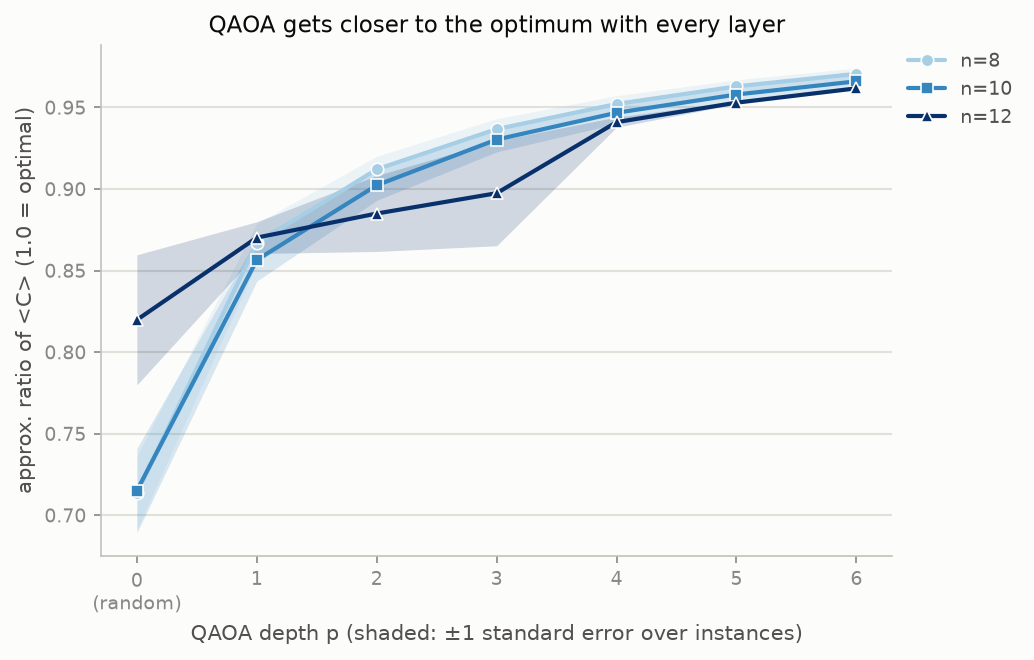
\includegraphics[width=0.8\linewidth]{E1_approx_ratio.png}\\[6pt]
  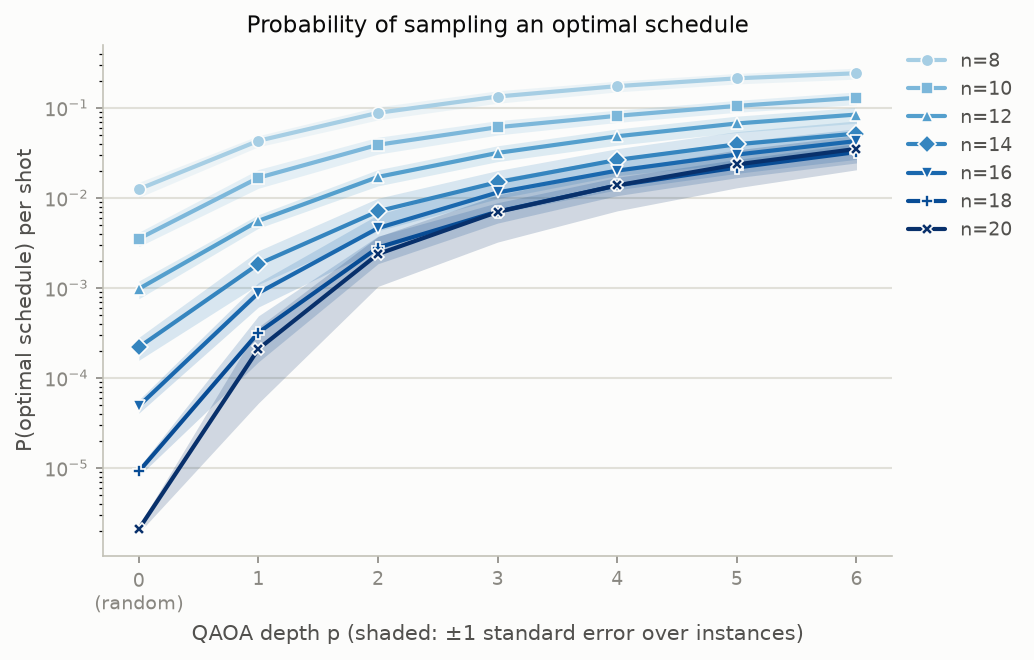
\includegraphics[width=0.8\linewidth]{E1_p_opt.png}
  \caption{E1. Top: approximation ratio of the mean cost against depth. Bottom: probability that one shot is optimal (log scale). $p = 0$ is random guessing.}
  \label{fig:e1}
\end{figure}

Quality improves with every layer (Fig.~\ref{fig:e1}, top): from $0.71$--$0.73$ for random guessing to $0.83$--$0.87$ at $p = 1$ and $0.93$--$0.97$ at $p = 6$.
No instance ever got worse with depth, but the gains shrink: at $n = 8$ layer 2 adds $0.045$ and layer 6 only $0.008$.
The dip at $n = 14$ and $16$ comes from two instances whose INTERP chain is stuck at $r \approx 0.73$ from $p = 1$ onwards; transferred angles reach $0.96$ and $0.92$ on them (E2), and without them both sizes average $0.95$.

$P(\text{opt})$ at $p = 6$ falls from $0.24$ at $n = 8$ to $0.035$ at $n = 20$ (Fig.~\ref{fig:e1}, bottom), but random guessing falls as $2^{-n}$, so QAOA's advantage grows from 19 to about $17{,}000$ times.
From $p = 3$ the best of 10{,}000 shots is an exact optimum on all 70 instances.
Single-precision GPU runs stop after about half as many COBYLA evaluations as CPU runs at the same quality, so we compare evaluation counts only within one precision.
